\documentclass[letterpaper]{article}
\usepackage[margin=1in]{geometry}

\usepackage{graphicx} % allows graphics
\usepackage{caption}  % modify caption width
\usepackage{subcaption}  % use subfigure environment

\usepackage{biblatex} %Imports biblatex package
\addbibresource{bibliography.bib} %Import the bibliography file

\usepackage{verbatimbox} % create figures with verbatim/code text

\usepackage{lmodern}
\renewcommand*\familydefault{\sfdefault} %% Only if the base font of the document is to be sans serif
\usepackage[T1]{fontenc}

\usepackage{xcolor} %% custom colors for hyperref
\definecolor{darkergrey}{rgb}{0.35,0.35,0.35}

\usepackage{hyperref} %% turn links, references in to hyperlinks
\hypersetup{
	colorlinks=true,
	linkcolor=darkergrey,   
	urlcolor=darkergrey,
	citecolor=darkergrey
}

%opening
\title{A Web Application for Manually Tracking Locational Event Data in Ice Hockey}
\author{An Nguyen\thanks{Harvey Mudd College; \href{mailto:anguyen@hmc.edu}{anguyen@hmc.edu}}}
\date{}
\begin{document}

\maketitle

\begin{abstract}
Sometimes, sports data must be tracked by hand, as desired data may not be available through existing sources, if it exists at all. But, manual tracking is often tedious and hard to translate into a useful form for analysis. In ice hockey, manual tracking is often especially necessary in women’s and youth ice hockey as data is often sparser and more difficult to access in those competitions. To aid the process of manual tracking in ice hockey and encourage an increase in the breadth and depth of data available, this work describes an open-source web application designed to reduce the hardships of manually tracking locational event data in ice hockey. The web application distinguishes itself from similar applications by its user-friendliness and high level of customizability. By clicking on a location on a rink, the corresponding coordinates of that event are logged as a table row. Details in additional columns in the table are recorded using a details panel beside the rink. The data is downloadable in \texttt{.csv} format for further exploration and analysis. New details can be created with corresponding widgets in the details panel and columns in the table. The application also provides the ability to record one or two sets of coordinates per event, for tracking events where start and end locations are desired. These custom setups of the application with new details and options can be saved and later loaded into the web application, saving time recreating the environment.
\end{abstract}

\section{Introduction}
\subsection{What is the Web Application?}
The web application (\href{https://shot-plotter.netlify.app/}{shot-plotter.netlify.app}) provides a graphical interface for creating a table of events occurring during an ice hockey game. Coordinates are logged by clicking on the appropriate location on a rink. Additional details about the event are recorded in a details panel beside the rink using form elements like radio buttons, text fields, and dropdowns. The event table is then downloadable in \texttt{.csv} format. The app is currently known as \textit{Shot-Plotter} due to its original and default purpose of plotting shots; however, its customizability enables tracking any events and associated details with ease.

\subsection{Prior Work}
Over the past few years, there have been various web applications with the same core idea of providing a graphical interface of a clickable rink for logging locational events in ice hockey.

At the start of 2018, the now-defunct tracking system, \textit{Tape to Tape} was released by Rushil Ram in conjunction with hockey analytics website Meta Hockey \cite{tapetotape}. \textit{Tape to Tape} was specifically designed for tracking passes, zone entries, and zone exits in the NHL. \textit{Tape to Tape} had unique features catered to that purpose like integration with the NHL play-by-play data, but was not accomodating to other use cases.

In late 2018, inspired by a podcast comment by Alyssa Longmuir about useful tools for a "'grassroot' analytics league" outside of the NHL, Andrew Pucci released \textit{ShotPlot} \cite{alyssaAustraliaArticle}. \textit{ShotPlot} \cite{shotplot} hones in on the location-recording aspect of tracking events: the application allows custom units of measurement (i.e. feet, meters, etc.) and provides the ability to toggle between the different specifications of a North American rink and an international rink. However, no additional details about events can be recorded using \textit{ShotPlot}.

Longmuir used a mix of hand tracking and \textit{ShotPlot} for tracking a season of the Australian Women's Ice Hockey League. But when she wanted to have shot heat maps on hand for helping local teams perform and schoolchildren get into sports analytics, Longmuir developed her own application, \textit{Hockey Plotter} in late 2020 \cite{alyssaShinyArticle}. \textit{Hockey Plotter} \cite{alyssaWebsite} is a Shiny application that features a rink to plot shots or goals, as well as radio buttons and a text field to log the team and player of each event, respectively. Its most unique feature was the cause of its creation: by switching tabs in the application, plotted shots are visualized as a heat map. However, a key drawback is the slowness of plotting shots: after clicking on the rink, each shot takes a second or two to appear.

After using Longmuir's \textit{Hockey Plotter} to help digitize shot charts from historical women's ice hockey Olympics games and being frustrated by the shot-appearance delay,  \textit{Shot-Plotter} was originally released in early April 2021.

\subsection{What Makes Shot-Plotter Unique}
What sets \textit{Shot-Plotter} apart is two-fold: its ease of use and adaptability. 

The application prioritizes having a straightforward user interface (UI) and having as little friction while using the application as possible. Events appear instantly after clicking on the rink to provide immediate feedback to the user. The UI is responsive, adapting to changes in screen size for compatibility with computers and mobile devices. The application is functional with the default setup, without forcing a need for customization if not desired. If users wish to customize the application, the UI guides the user using form elements, examples, and labels. Documentation is hidden by default to avoid overwhelming the user with information but is available if needed.

The most noteworthy feature of \textit{Shot-Plotter} is the degree of customization users have, especially with regards to additional details logged alongside the coordinates. Similar applications have fixed options for information recorded alongside coordinates, while \textit{Shot-Plotter} allows deleting, reordering, and adding new additional details. Combined with the ability to record two sets of locations per event, \textit{Shot-Plotter} can be used to track almost any event and associated details imaginable. The application is also agnostic of the league, competition, and level of ice hockey. Theoretically, any event occurring on an ice rink is trackable with \textit{Shot-Plotter}.


\section{The Structure of the Application}

\begin{figure}[h!]
	\centering
	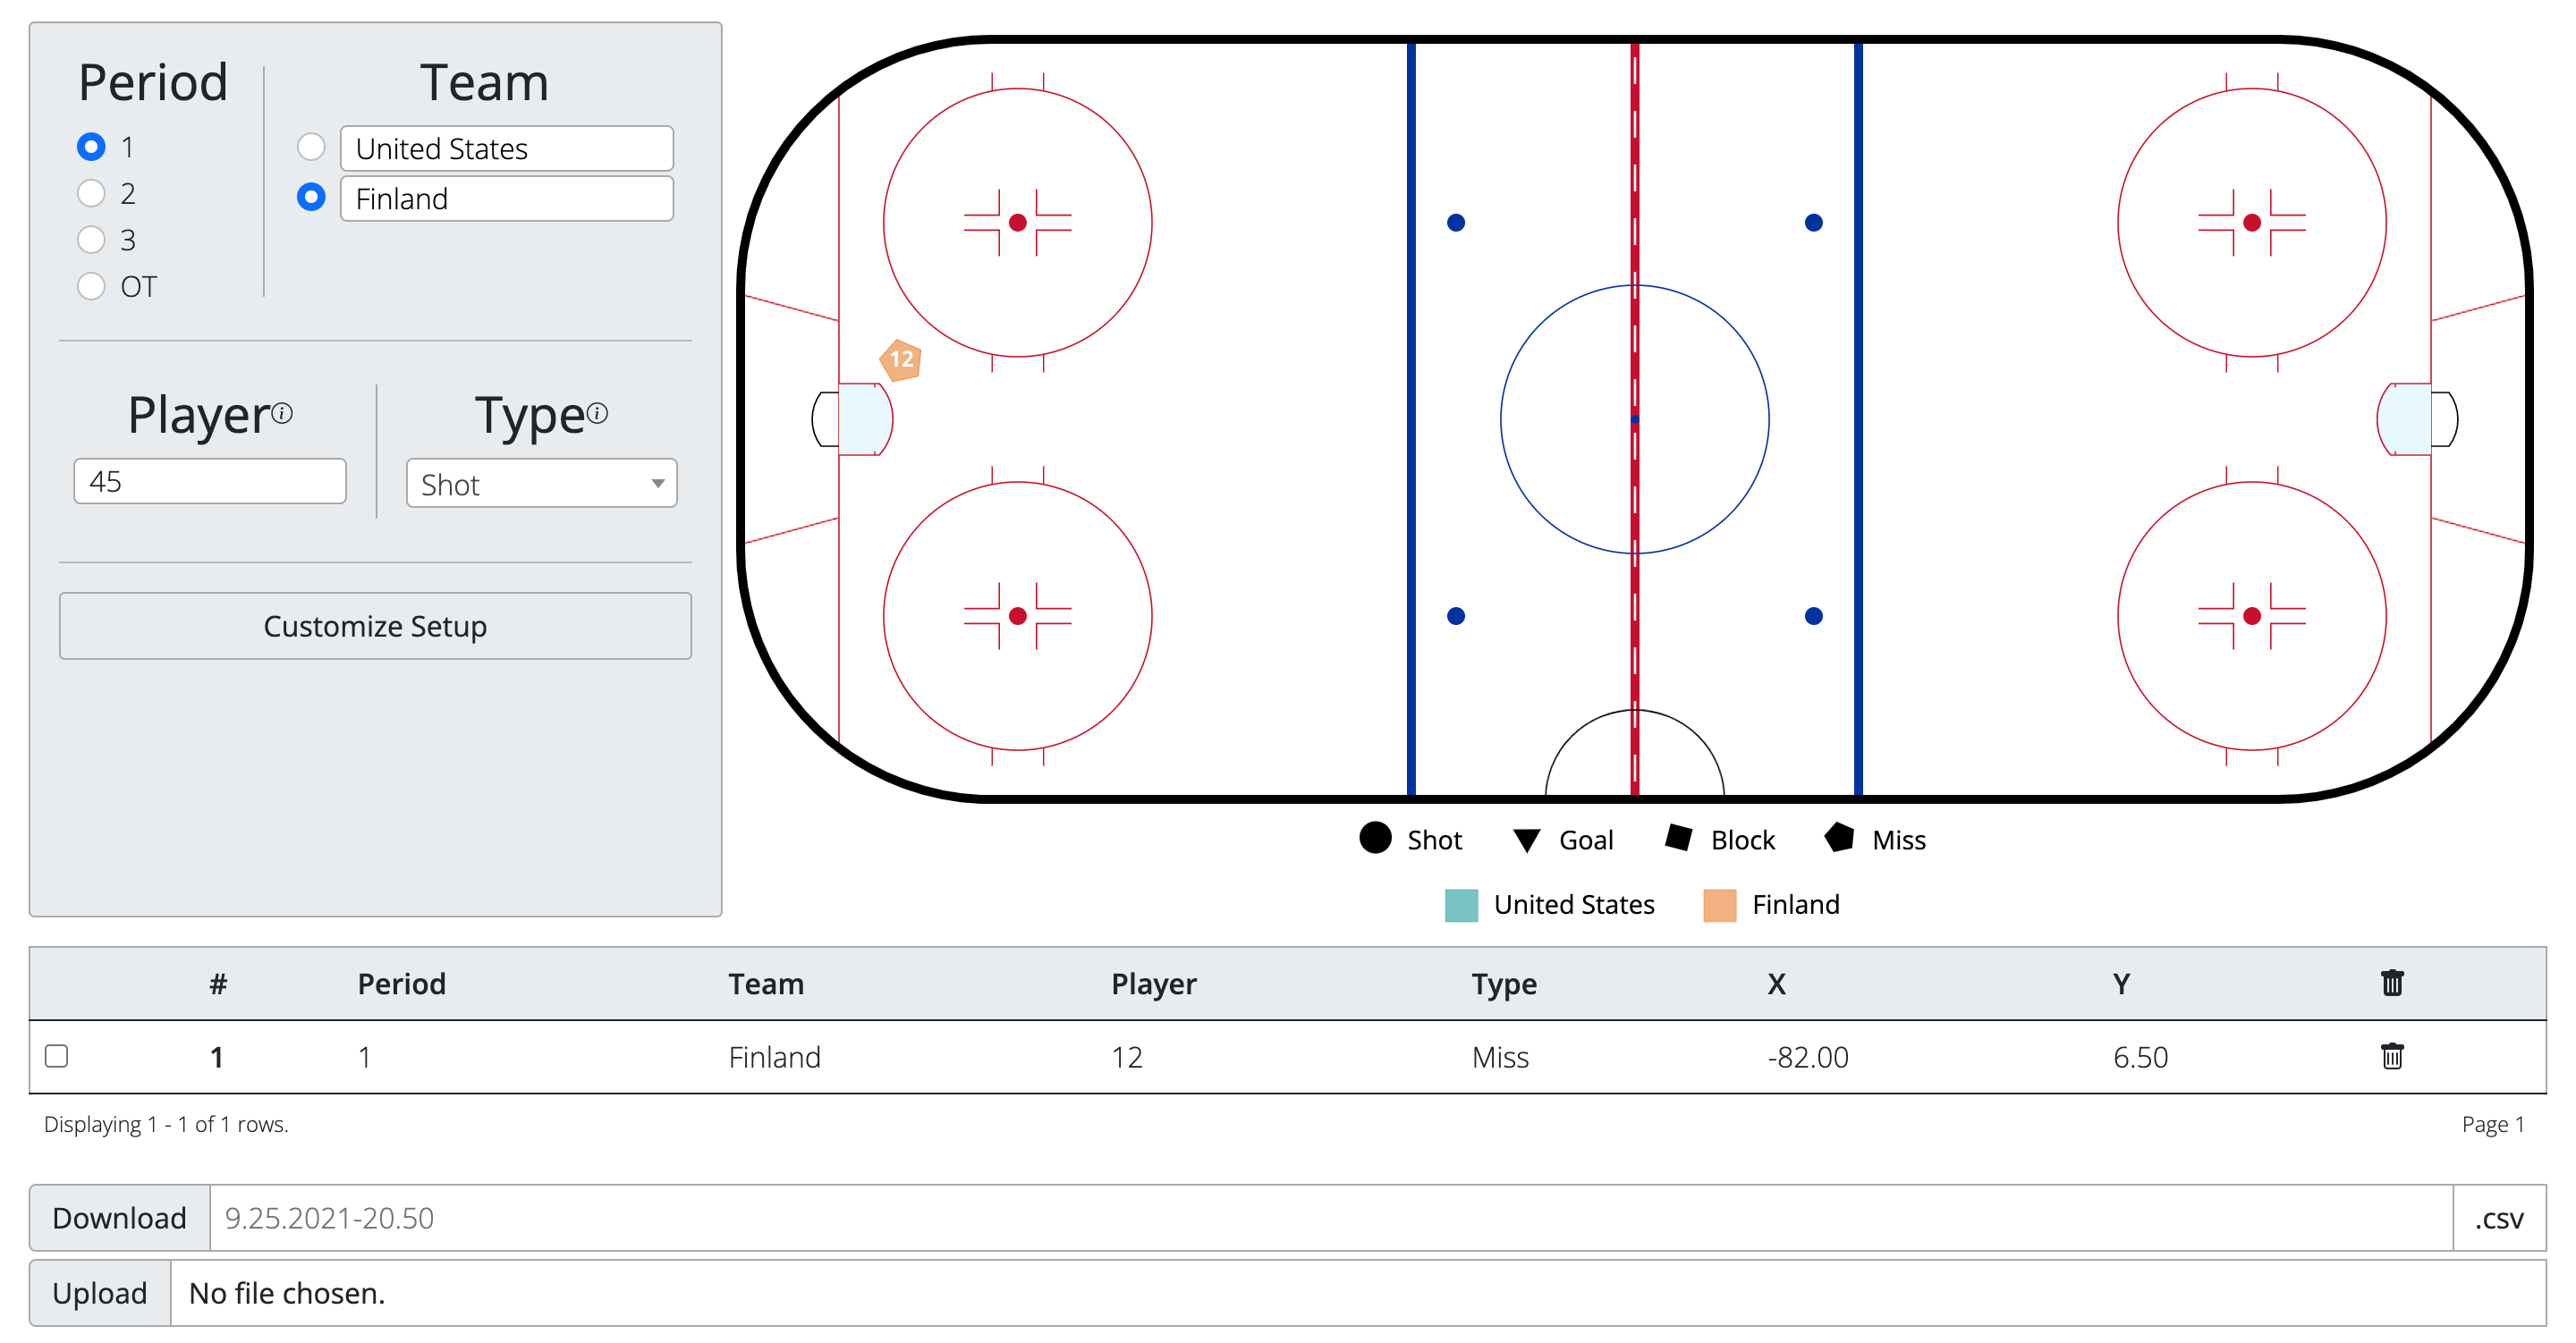
\includegraphics[width=1\linewidth]{images/full-screenshot}
	\caption{A screenshot of the \textit{Shot-Plotter} web application, with the header and footer cropped to save space. A rink (Section \ref{rink}) and a details panel (Section \ref{sidepanel}) to the left occupy most of the space. Below the details panel and rink is a table (Section \ref{table}) containing one row. Below the table is a section to upload and download the table (Section \ref{table-up-down}).}
	\label{fig:full-screenshot}
\end{figure}
\subsection{Rink}\label{rink}
Clicking on the rink logs an event.

The rink matches the NHL rulebook specifications as of the 2021-2022 season \cite{nhlrulebook} and the coordinate system matches that of NHL play-by-play data. The center of the rink has coordinates (0,0). The x-axis is along the length of the rink; x-values range from -100 feet on the left to 100 feet on the right. The y-axis is along the center line of the rink; y-values range from -42.5 feet at the bottom to 42.5 feet at the top.

When the rink is clicked, a row in the table appears and a dot appears at the clicked location. These comprise a representation of the event logged. Additional details about the event included in the row, as well as the dot's appearance, are based on the information in the details panel (Section \ref{sidepanel}).

\subsection{Details Panel}\label{sidepanel}
The details panel is where additional details about an event are recorded. 

The details panel is divided into sections called widgets that provide a way to record additional details for each event. When an event is logged by clicking on the rink, the value of the event's row in each detail column is the current value of the corresponding detail widget. For example, in Figure \ref{fig:full-screenshot}, since the value "Shot" is currently selected in the \textbf{Type} widget, if an event were to be logged, the value in the \textbf{Type} column would be "Shot".

The default details, \textbf{Period}, \textbf{Team}, \textbf{Player}, \textbf{Type}, were chosen as common information wanted for a shot in ice hockey. The default details (excluding \textbf{Period}) also map to specific visual indicators on the rink. The \textbf{Team} and \textbf{Type} details control the color and shape of the event's dot on the rink, respectively; the legend below the rink indicates the corresponding values. The legend updates as the \textbf{Team} names are edited and additional options are added to \textbf{Type}. If the value in the \textbf{Player} widget is two characters or less (intended for indicating a player's number), the value will appear on the dot. These visual indicators increase the legibility of events just from the rink and minimize the need to cross-reference with the table. For example, in Figure \ref{fig:full-screenshot}, we can determine the logged event on the rink was a "Miss" by "Finland" player number "12" just by looking at the dot.

\subsection{Table} \label{table}
The table displays the event information in a layout that mimics the downloadable version of the data and allows the highlighting and deletion of events.

By default, the table has 7 columns: 4 corresponding to the widgets, \textbf{Period}, \textbf{Team}, \textbf{Player}, \textbf{Type},  an \textbf{X} and \textbf{Y} column for the x-coordinate and y-coordinate of the event's location, and a \textbf{\#} column indicating the number of the event relative to the other events (i.e. the fifth event logged has value "5" in the \textbf{\#} column).

The table is divided into pages of rows; by default, the table shows the last page, which contains the last ten events recorded. The footer of the table indicates the numbers of the currently displayed events on the left-hand side; the right-hand side of the footer shows the current page and has buttons for switching to the previous and next page of the table, if any (Figure \ref{fig:highlighting}).

On the left end of each event's row in the table, there is a checkbox that is used to highlight that event. When an event is highlighted, its row is colored corresponding to its team, and its dot on the rink enlarges. Multiple events can be highlighted at once (Figure \ref{fig:highlighting}).

There is a trash can icon on the right end of each event's row. When clicked, that event is deleted: the corresponding row and dot disappear from the table and rink respectively, and the event numbering in the \textbf{\#} column adjusts if needed. There is also a trash can icon alongside the column names in the table; when clicked, a modal appears asking if the user wants to delete all recorded events. If the user confirms, all rows and dots disappear from the table and the rink.

\begin{figure}[h!]
	\centering
	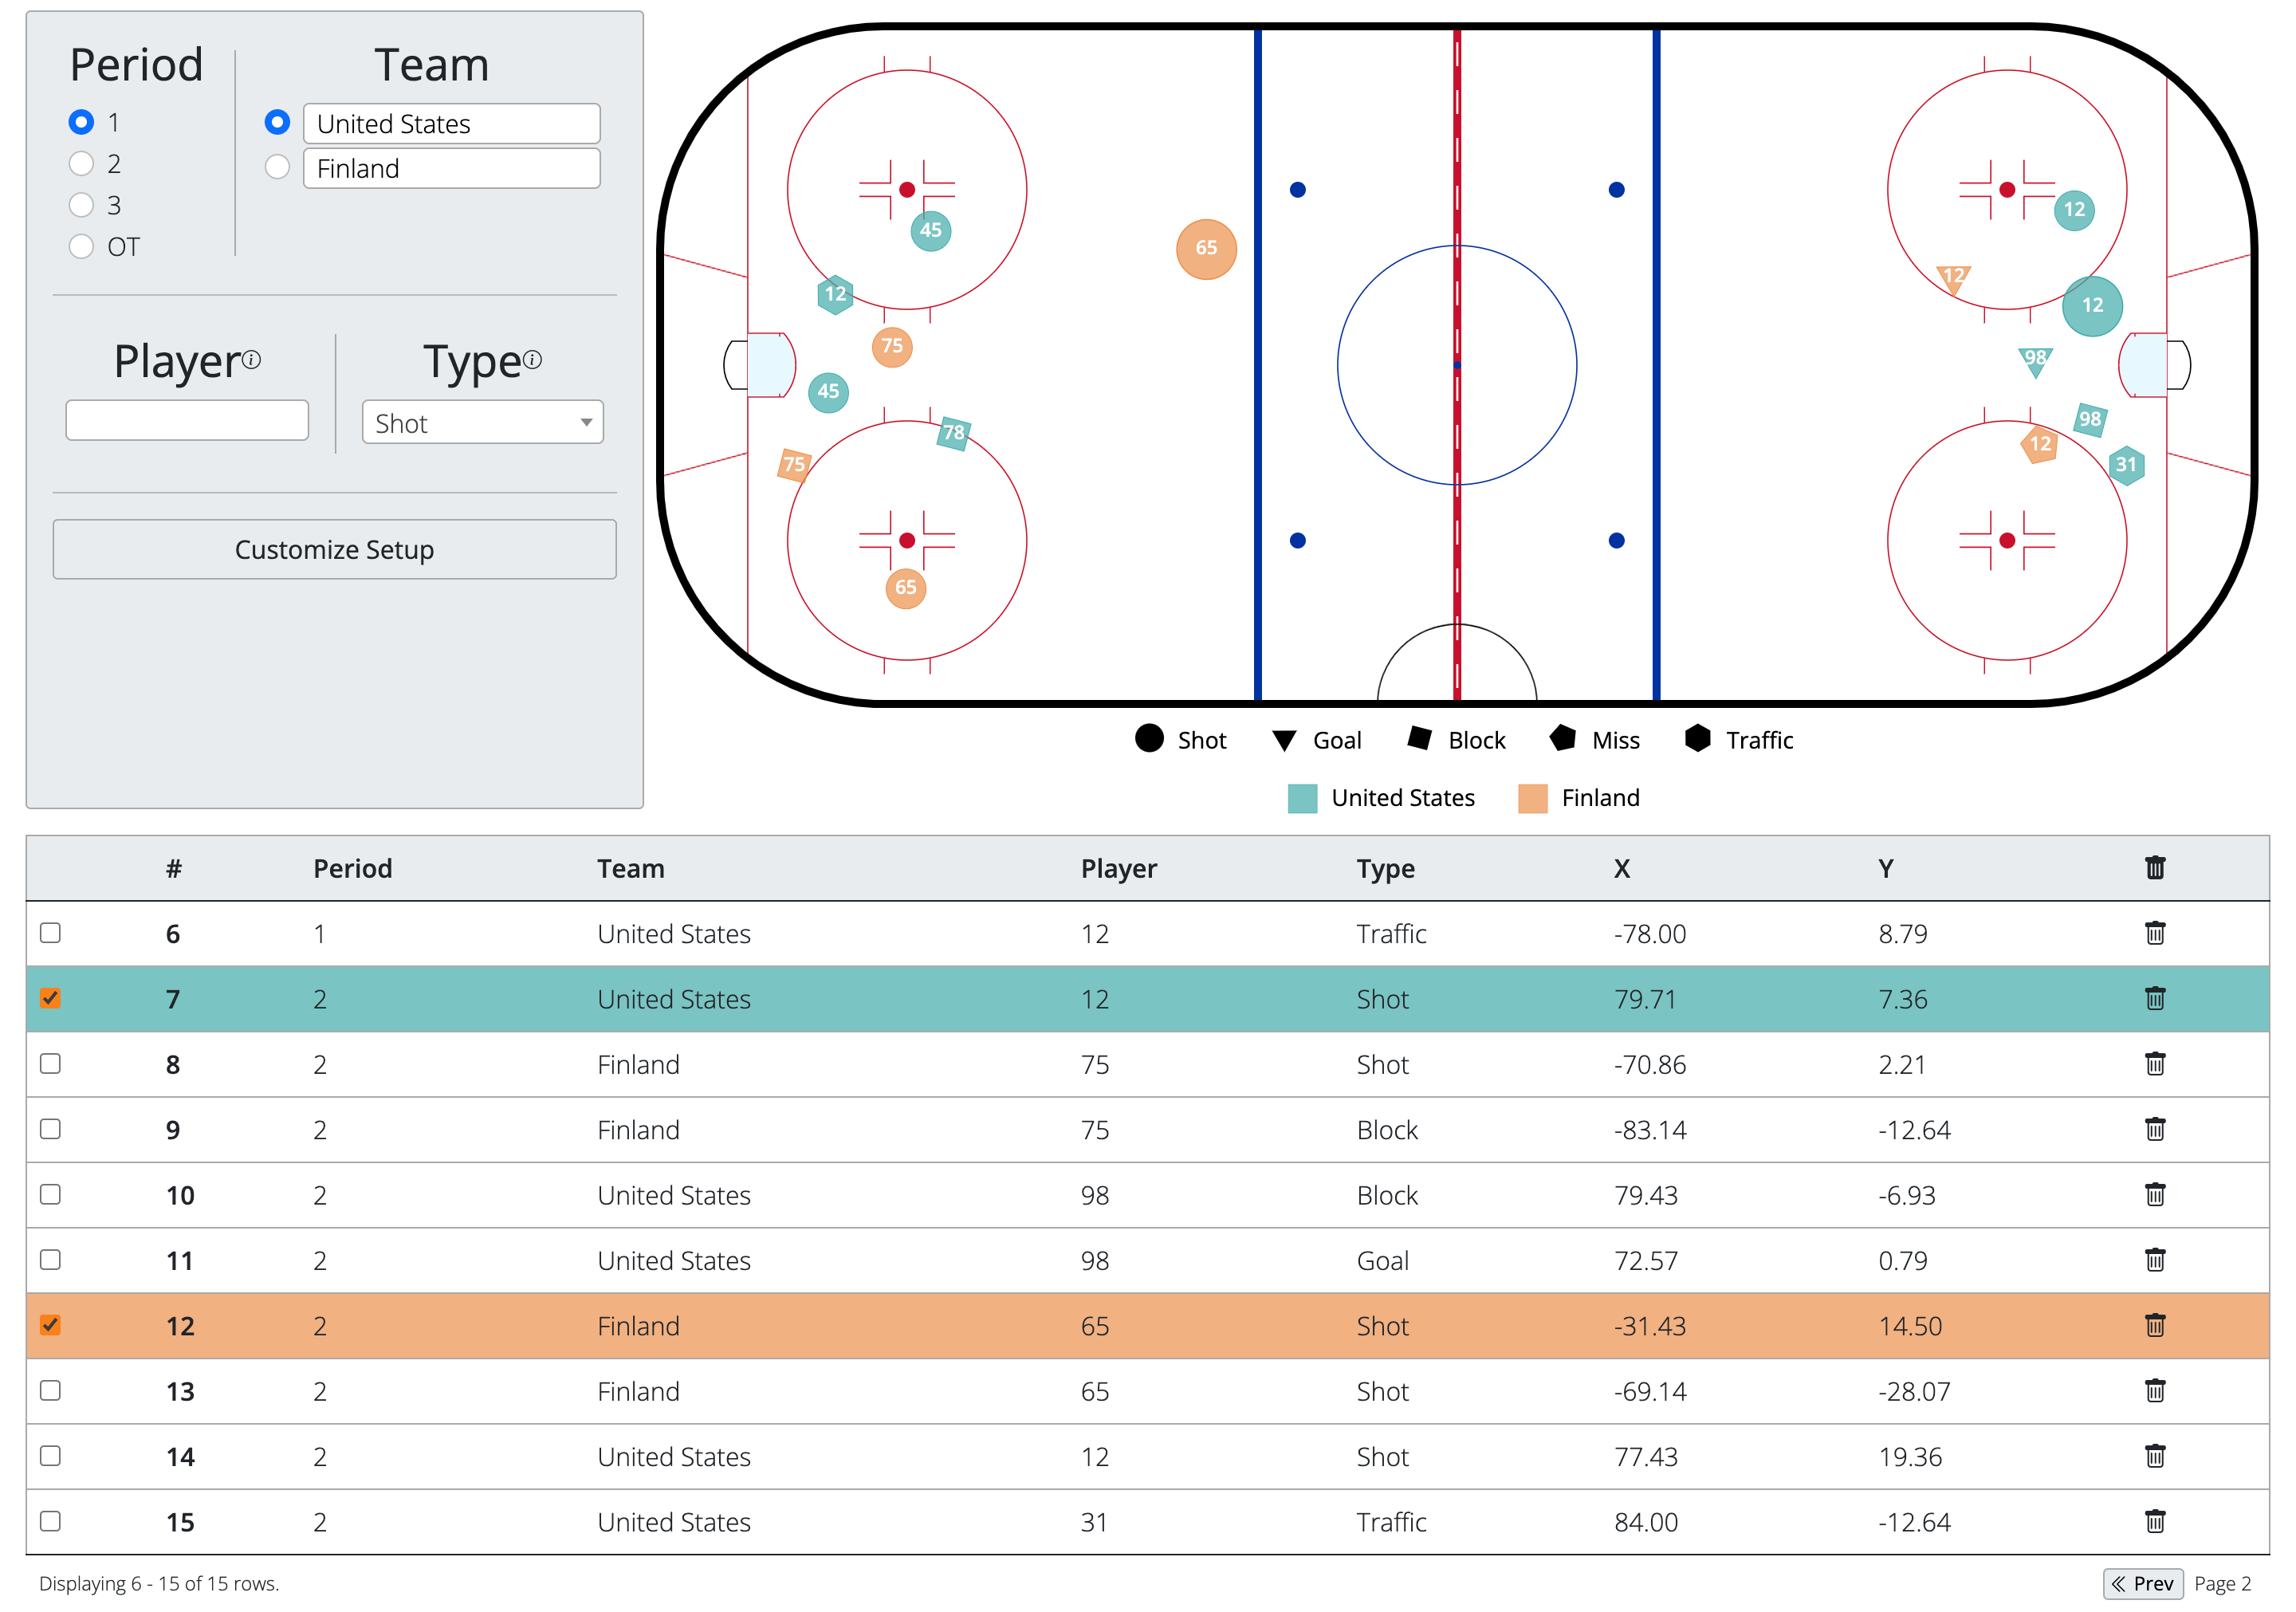
\includegraphics[width=1\linewidth]{images/highlighting}
	\caption{A screenshot of the \textit{Shot-Plotter} web application; the header, footer, and table download and upload functionality are cropped out to save space. Only the 6th through 15th events out of 15 total events are currently displayed in the table, per the footer. There is a button to navigate to the previous page of the table. The table contains two highlighted events. On the rink, the larger size of the highlighted event dots distinguishes between the two "Shot" events by "United States" player "12" on the right half of the rink and between the two "Shot" events by "Finland" player "65" on the left half of the rink, which otherwise would appear identical.}
		\label{fig:highlighting}
\end{figure}

\subsection{Table Download and Upload}\label{table-up-down}
Below the table is a section where the table can be downloaded in \texttt{.csv} format, or the table can be populated by uploading an existing \texttt{.csv}.

Typing into the white text box between the download button changes the file name, though it is always in \texttt{.csv} format as indicated at the end. By default, the file name is the date and time when the web app was initially opened.

The downloaded file includes the values in any columns with corresponding widgets in the details panel and any coordinate columns; this means the default \textbf{\#} column is excluded. The downloaded file includes column names. Figure \ref{fig:csvoutput} shows the contents of the downloaded \texttt{.csv} file corresponding to the table in Figure \ref{fig:full-screenshot}.

Files can be uploaded by clicking anywhere on the upload section; files must be in \texttt{.csv} format with column names in the file corresponding to the widget and coordinate column names in the web application's table. When a file is uploaded, any events currently in the app's table are removed, and then the table and rink populate with rows and dots corresponding to the events in the file.

\begin{verbbox}
	Period,Team,Player,Type,X,Y
	1,Finland,12,Miss,-82.00,6.50
\end{verbbox}
\begin{figure}[ht]
	\centering
	\theverbbox
	\caption{Content of a downloaded \texttt{.csv} file corresponding to the table in Figure \ref{fig:full-screenshot}.}
	\label{fig:csvoutput}
\end{figure}
\subsection{Sample Workflow using the Default Application}
What follows is an example of a possible workflow to illustrate features in action using the default setup of the application.

Say we are tracking shot events for a game between Sweden and Germany. Before the game starts, we can enter "Sweden" and "Germany" into the name boxes in the \textbf{Team} widget; the countries will then appear in the color legend below the rink. We can also add any additional values we want to the \textbf{Type} widget to not waste time typing them when they come up in-game. If we wish to distinguish shots through traffic, for example, we can add the value "Traffic" to the \textbf{Type} widget by typing it into the dropdown and hitting enter. "Traffic" will then appear as a new option in the dropdown and the shape legend beneath the rink.

Then, when the game starts, we can track shots as they happen, adjusting the \textbf{Player} and \textbf{Type} values as necessary in the details panel and then clicking on the matching location on the rink to log the shot. We will likely make mistakes along the way: perhaps we click on the wrong location or forget to adjust one of the details. In that case, we can delete the erroneous shot from the table and then log it again. If we figure out we erred logging an older shot, we can highlight events to ensure we delete the intended one. We can also highlight events throughout the game to keep track of key shots we want to note later.

Say we get to the break between periods 1 and 2. After switching the \textbf{Period} widget value to "2", we might want to save our progress. We can download the shots currently in the table to a \texttt{.csv} file, naming it \texttt{germany-sweden-period-1.csv} to indicate it is not a complete game tracking. After we download the file, the events are still in the web application table. We can then continue tracking shots in the following periods, adding to the logged shots from period 1. Alternatively, we can use the trash can icon in the table header to delete all current shot events and instead track period 2 using a clean rink and table while preserving our values in the details panel, and then merge the files later. Either way, if anything happens, we can upload our downloaded file to restore all of the tracked events from the first period.

Then, when the game is over, we can download our \texttt{.csv} file(s) and use them for statistical analysis, either by hand or with some other tool.

\section{Customizing the Setup of the Application}
By default, the \textit{Shot-Plotter} application is aimed at tracking shots. However, by customizing the application's setup, the app can be tailored to any use case. Customizing the setup can involve changing what additional details are recorded with each event (Sections \ref{reorder-hide-delete} and \ref{create-column}), modifying the application's appearance (Section \ref{modify-appearance}), and enabling 2-location events (Section \ref{two-location}). These custom setups can be downloaded to a file and restored at a later point by uploading that file (Section \ref{setup-download-upload}).

The setup can be customized by clicking on the "Customize Setup" button at the bottom of the details panel. The setup can only be customized when there are no events logged; when events are logged, the "Customize Setup" button turns grey to indicate it is disabled.

Clicking on the "Customize Setup" button causes a pop-up window to appear (Figure \ref{fig:main-page}). At the top, there is a quick blurb about what options are available, with a "More Info" option that, when clicked, expands to display more detailed instructions on how to achieve everything mentioned. The "Save Changes" button in the bottom right closes the pop-up, returning the user to the main application but with any customizations applied.

\begin{figure}[h!]
	\centering
	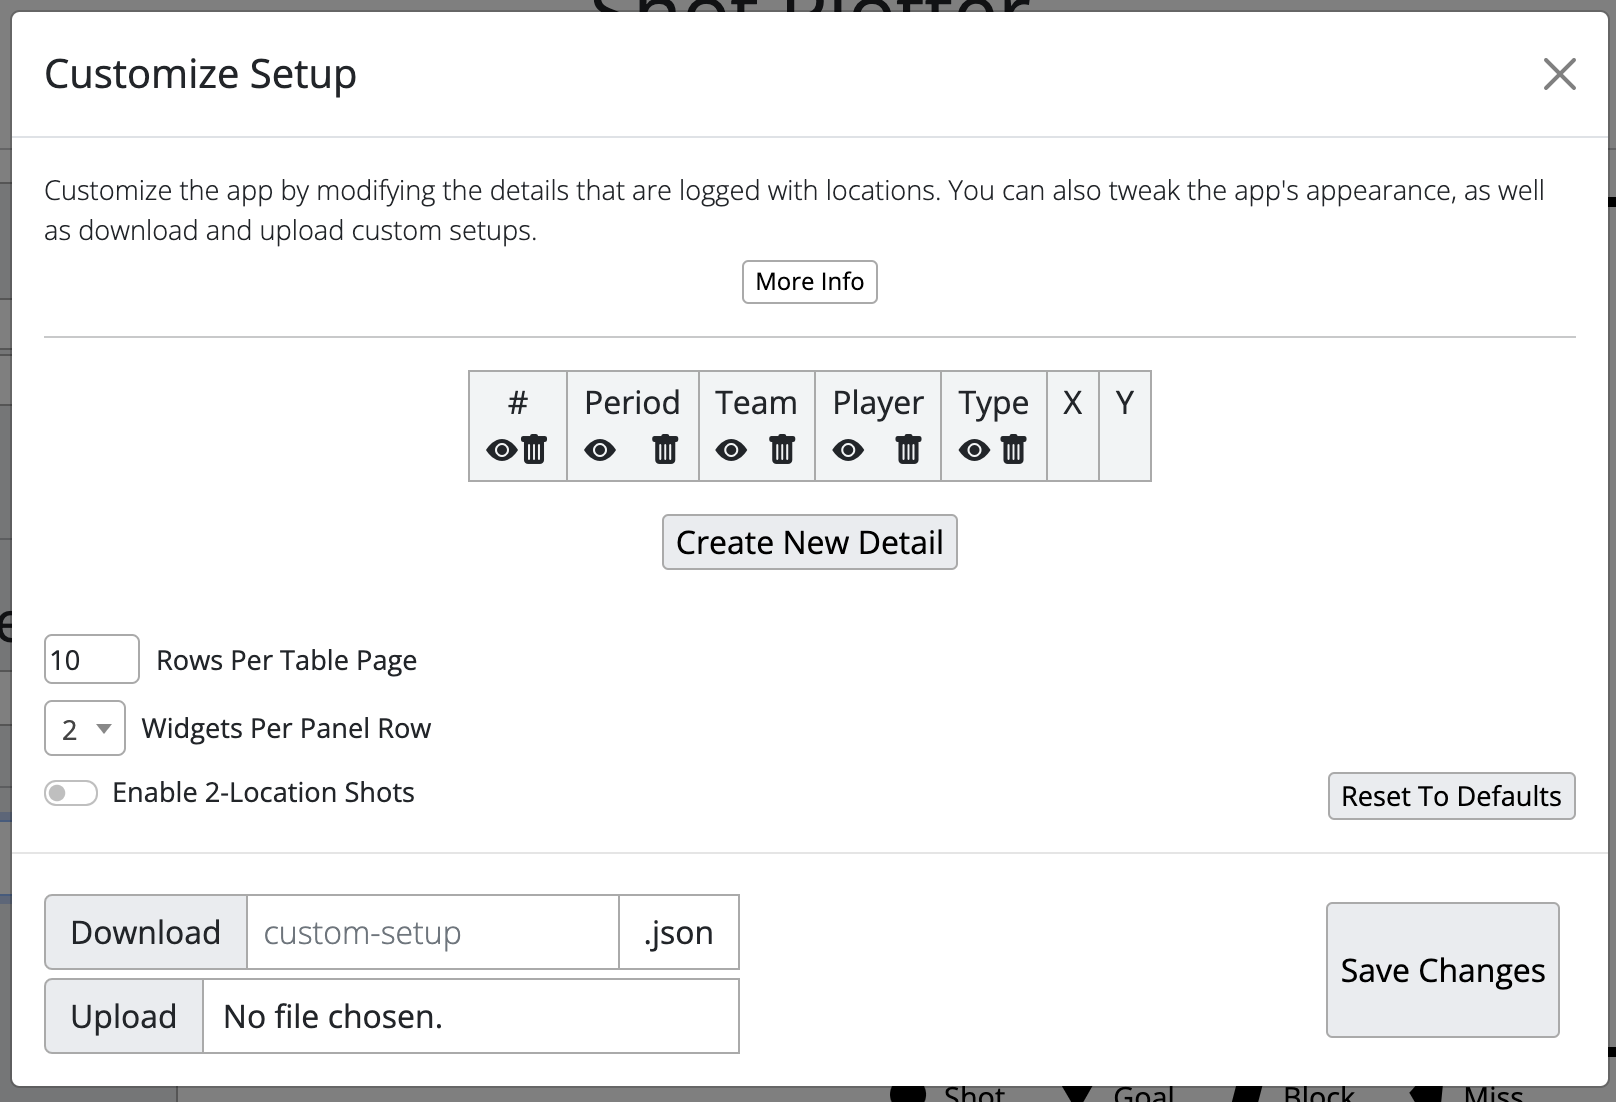
\includegraphics[width=1\linewidth]{images/main-page}
	\caption{A screenshot of the main view of the customization pop-up window. At the top is information about what can be customized. Below that is a row of boxes corresponding to the details (Section \ref{reorder-hide-delete}), then a button to create a new detail (Section \ref{create-column}). Below that are some options to modify the appearance of the application (Section \ref{modify-appearance}) and a toggle to enable 2-location events (Section \ref{two-location}). At the bottom is a section to download and upload a custom setup (Section \ref{setup-download-upload}).}
		\label{fig:main-page}
	\end{figure}

\subsection{Reordering, Hiding, and Deleting Details}\label{reorder-hide-delete}
Below the informational blurb, there is a row of boxes; each box corresponds to a detail recorded for each event. We can use the boxes to modify these details.

Dragging and dropping the detail boxes changes the order in which the matching detail widgets appear in the details panel, and the order in which detail columns appear in the table.

For most detail boxes, there is an eye icon and a trashcan icon. The eye icon indicates that detail is currently visible. By clicking on the eye icon, the corresponding widget and column of that detail are hidden from view and do not appear in the details panel and table respectively.  The eye icon will change to an eye with a slash to indicate it is hidden. Clicking on the eye icon will toggle between states of hidden and visible. Clicking on the trash can icon deletes the detail entirely; the detail disappears from the detail boxes, and the detail does not appear in the details panel or table. Coordinate details, like \textbf{X} and \textbf{Y}, cannot be hidden or deleted.

For example, say we deleted the \textbf{Period} detail, hid the \textbf{Type} detail, and reordered the boxes so the \textbf{Team} detail came last. Then in the details panel, the \textbf{Team} widget would come after the \textbf{Player} widget, and the columns in the table would be, in order, \textbf{\#}, \textbf{Player}, \textbf{X}, \textbf{Y}, \textbf{Team} (Figure \ref{fig:default-changes}).


\begin{figure}[!t]
	\begin{tabular}[b]{cc}
		\begin{tabular}[b]{c}
			\begin{subfigure}{.5\textwidth}
				\centering
				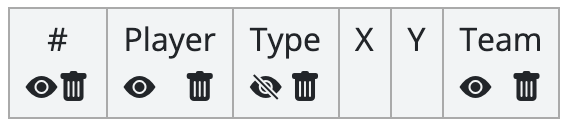
\includegraphics[width=.65\linewidth]{images/modified-row}
				\caption{A modified row of detail boxes.}
			\end{subfigure}\\
			\begin{subfigure}{.5\textwidth}
				\centering
				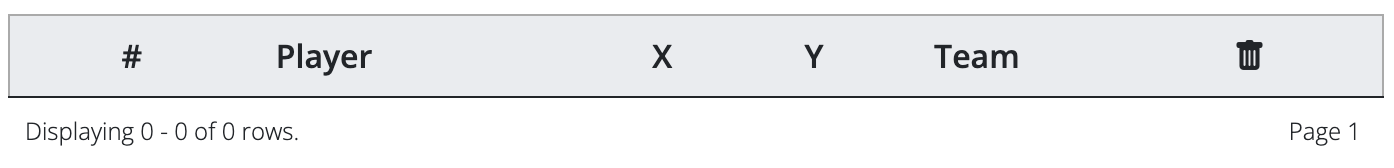
\includegraphics[width=1\linewidth]{images/modified-table}
				\caption{A modified table.}
			\end{subfigure}
		\end{tabular} &
		\begin{subfigure}{.42\textwidth}
			\centering
			\captionsetup{width=1\linewidth}
			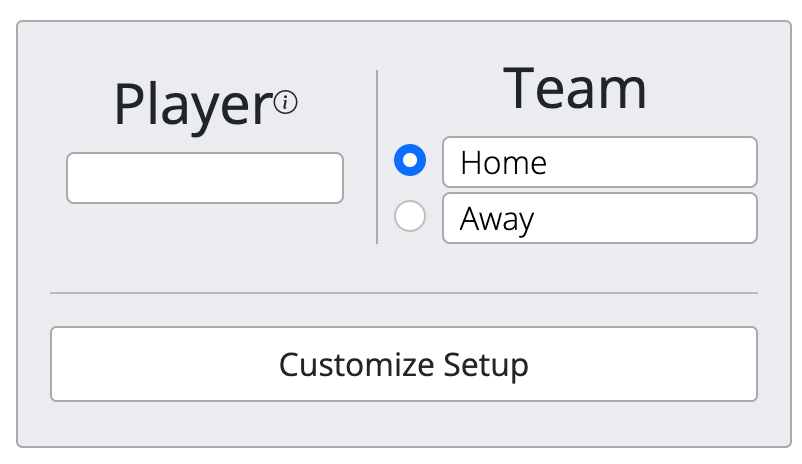
\includegraphics[width=1\linewidth]{images/modified-side-panel}
			\caption{A modified details panel (empty space cropped).}
		\end{subfigure}
	\end{tabular}
	\caption{The resulting changes to the detail boxes, details panel, and table produced by deleting the \textbf{Period} detail, hiding the \textbf{Type} detail, and reordering the columns so the \textbf{Team} detail comes last (Section \ref{reorder-hide-delete}).}
	\label{fig:default-changes}
\end{figure}

\subsection{Creating New Details}\label{create-column}
Say we want to record another detail for each event, \textbf{Strength}: whether an event occurs at even-strength, during a power play, or during a penalty kill. We can click on the "Create New Detail" button, and the customization pop-up window will switch to a view that describes the different kinds of detail widgets we can make (Figure \ref{fig:widget-select}).

\begin{figure}[h!]
			\centering
		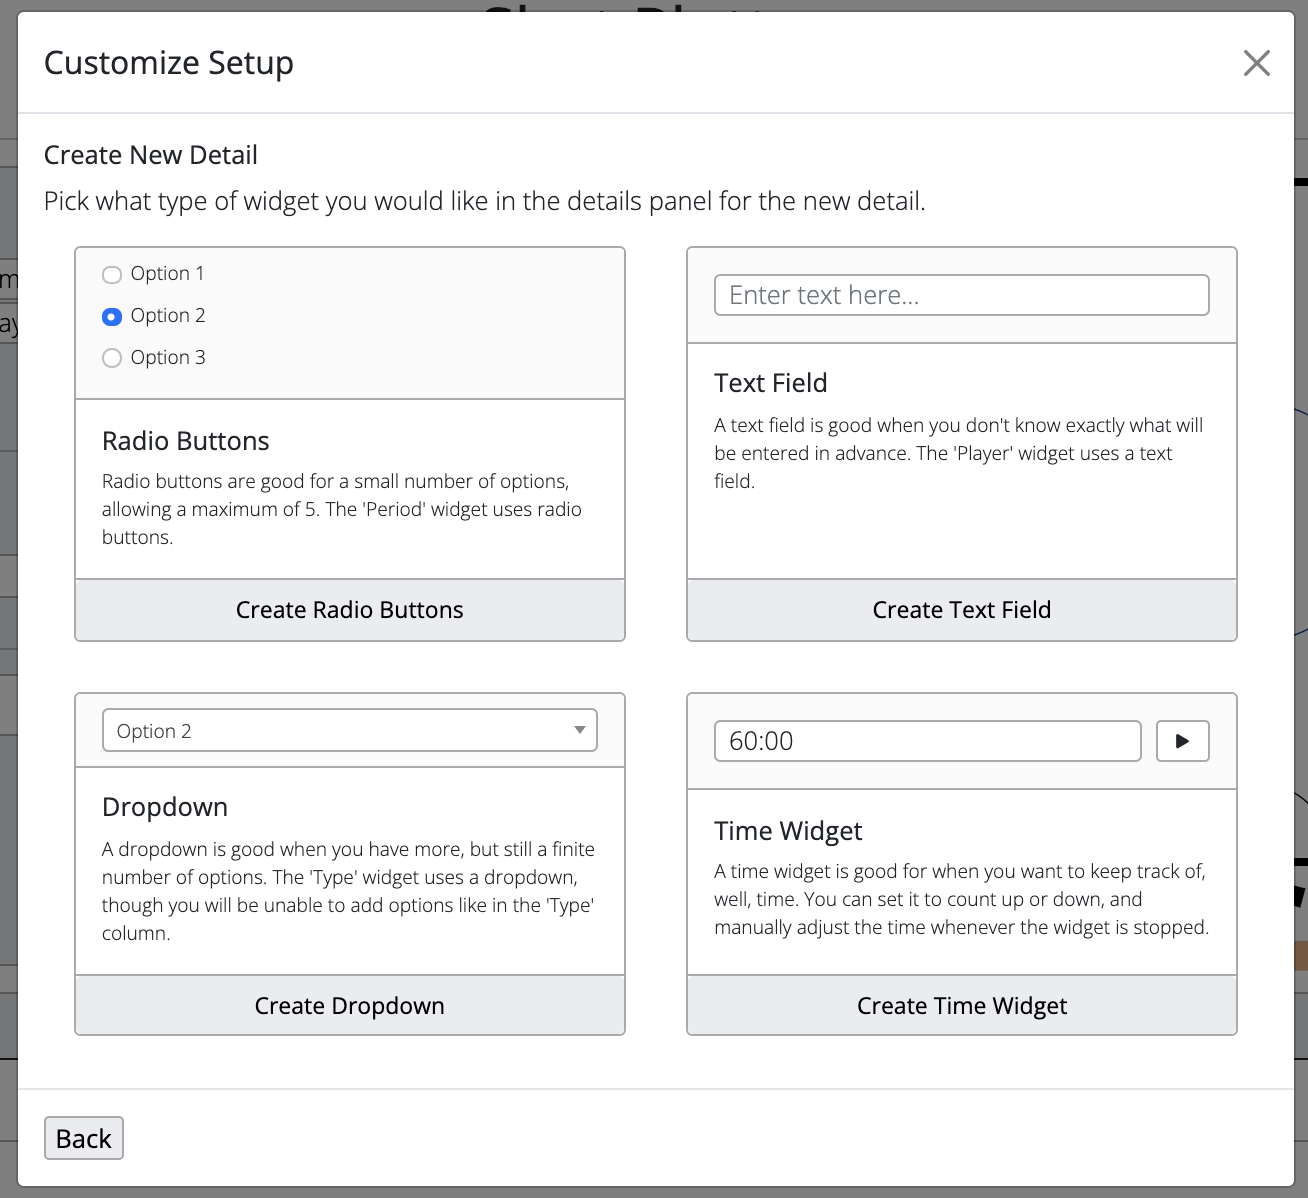
\includegraphics[width=.9\linewidth]{images/widget-select}
	\caption{A screenshot of the pop-up window view for selecting what kind of widget to create for a new detail.}
	\label{fig:widget-select}
	\end{figure}

\begin{figure}[h]
		\centering
	\captionsetup{width=.8\linewidth}
	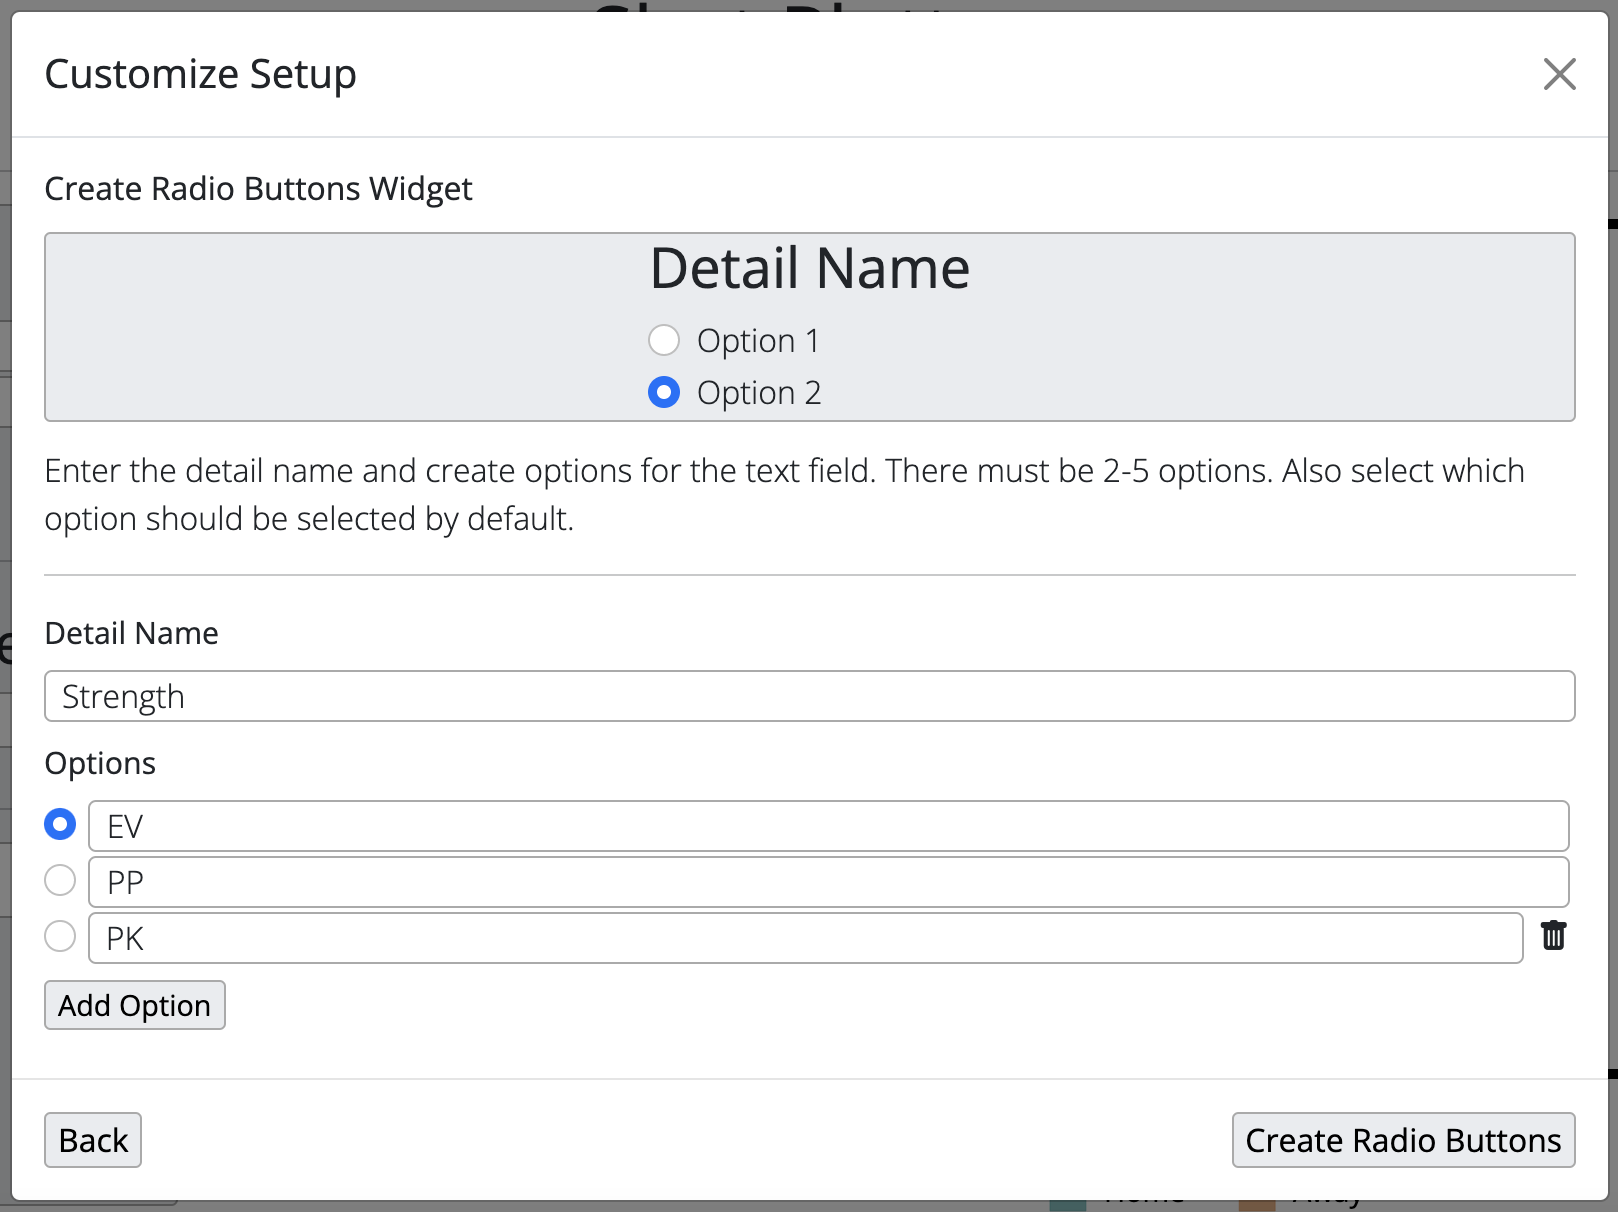
\includegraphics[width=.8\linewidth]{images/radio-buttons}
	\caption{A screenshot of the view for creating a new radio buttons widget. The form is filled out to create a new detail called \textbf{Strength} with options "EV", "PP", and "PK".}
	\label{fig:radio-buttons}
\end{figure}
New details can select from four types of widgets: radio buttons, text fields, dropdowns, and countdown/count-up timers (known as time widgets). For each widget, the view provides an interactive example and a brief description of ideal use cases. For \textbf{Strength}, since we only want three options, the descriptions suggest using radio buttons. We can click on the "Create Radio Buttons" button to switch to another view that guides us through creating our new radio buttons widget. Each widget type has a unique view for creating that widget; but all views have the same structure: an example at the top, a brief description of what is needed, and a form to enter the information for that widget. In our case, we can type "Strength" as the detail name,  and enter "EV" (even strength), "PP" (power play), and "PK" (penalty kill) as the options. We will need to add another option, as there are only two by default. We can then select "EV" to be the default selected option (Figure \ref{fig:radio-buttons}).

When we click "Create Radio Buttons," we are returned to the initial view of the customization window, but there is now a new detail box, "Strength" with a not-yet-seen pencil icon. The pencil icon allows editing that detail's widget: clicking it will return us to the radio buttons widget creation view, but the example will match the current widget and the form will be pre-filled appropriate for that widget. When we return to the main web application, we can see our new detail in action as a widget in the details panel and as a column in the table (Figure \ref{fig:strength-changes}).

Any number of new details can be created.

\begin{figure}[t]
	\begin{tabular}[b]{cc}
		\begin{tabular}[b]{c}
		\begin{subfigure}{.53\textwidth}
			\centering
			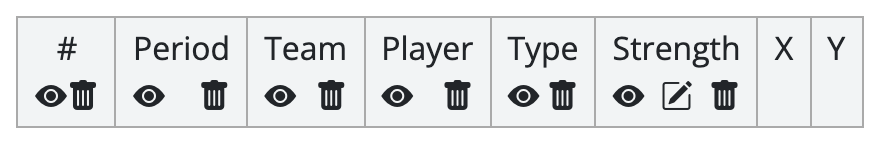
\includegraphics[width=1\linewidth]{images/strength-row}
			\caption{A row of detail boxes featuring the \textbf{Strength} detail.}
		\end{subfigure}\\
			\begin{subfigure}{.53\textwidth}
			\centering
			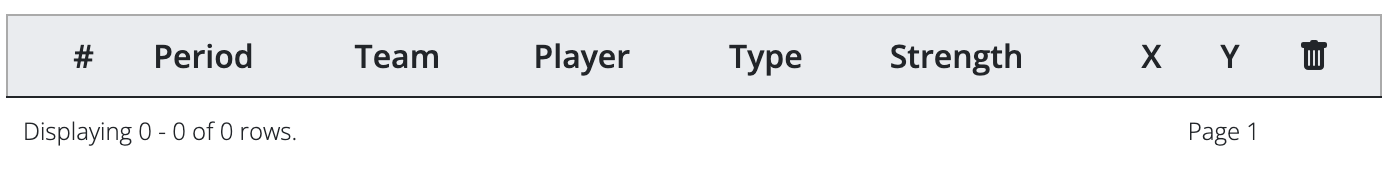
\includegraphics[width=1\linewidth]{images/strength-table}
			\caption{A table featuring the \textbf{Strength} column.}
			\end{subfigure}
		\end{tabular}
		&
\begin{subfigure}{.3\textwidth}
			\centering
			\captionsetup{width=1\linewidth}
			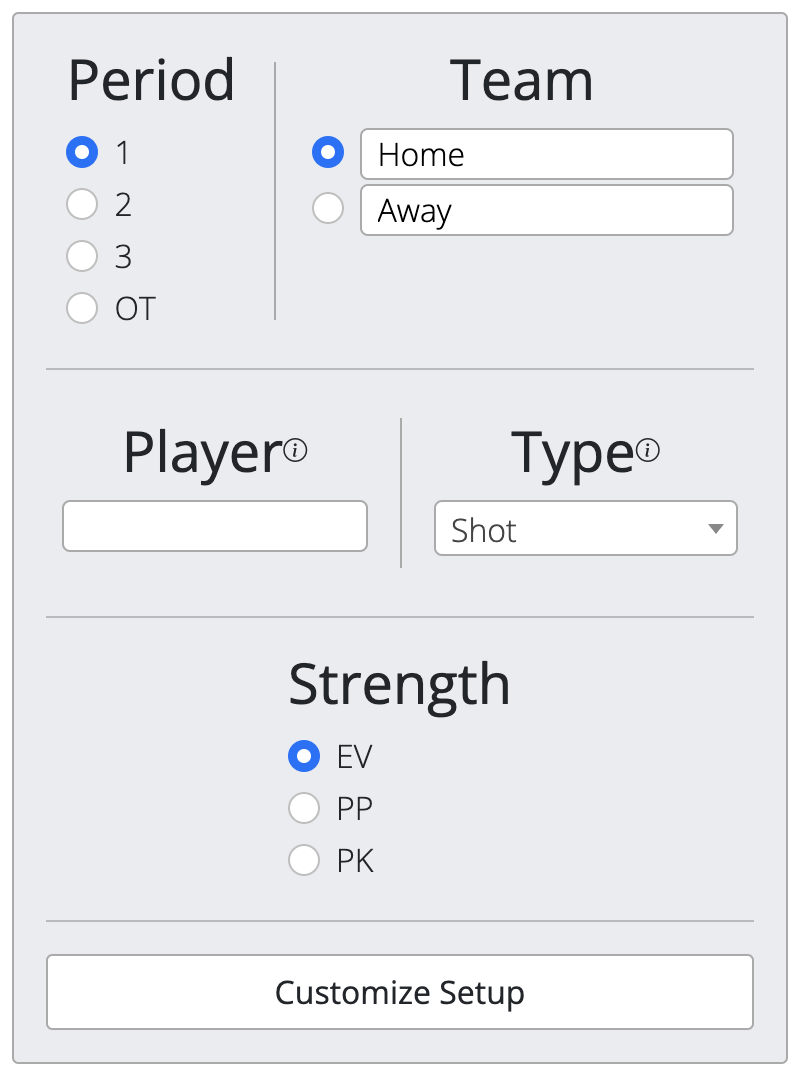
\includegraphics[width=1\linewidth]{images/strength-side-panel}
			\caption{A details panel featuring the \textbf{Strength} widget.}
		\end{subfigure}
	\end{tabular}
	\caption{The resulting changes produced by adding the \textbf{Strength} detail as described in Section \ref{create-column}.}
		\label{fig:strength-changes}
\end{figure}

\subsection{Appearance Preferences} \label{modify-appearance}
Below the detail boxes, on the left, there are options to modify the application's appearance.

By default, there are two widgets per row in the details panel; this number can be adjusted down to one, for users who want more space per widget, or up to three, for users who have many widgets and want to cut down on the space taken up by the details panel.

There are ten rows per page of the table by default. The number of rows can range from one row per page, for users who only want to see a single event at a time, all the way to 999, for users who want all events visible.
\subsection{2-Location Events} \label{two-location}

\begin{figure}[h]
		\begin{subfigure}{.5\textwidth}
	\centering
	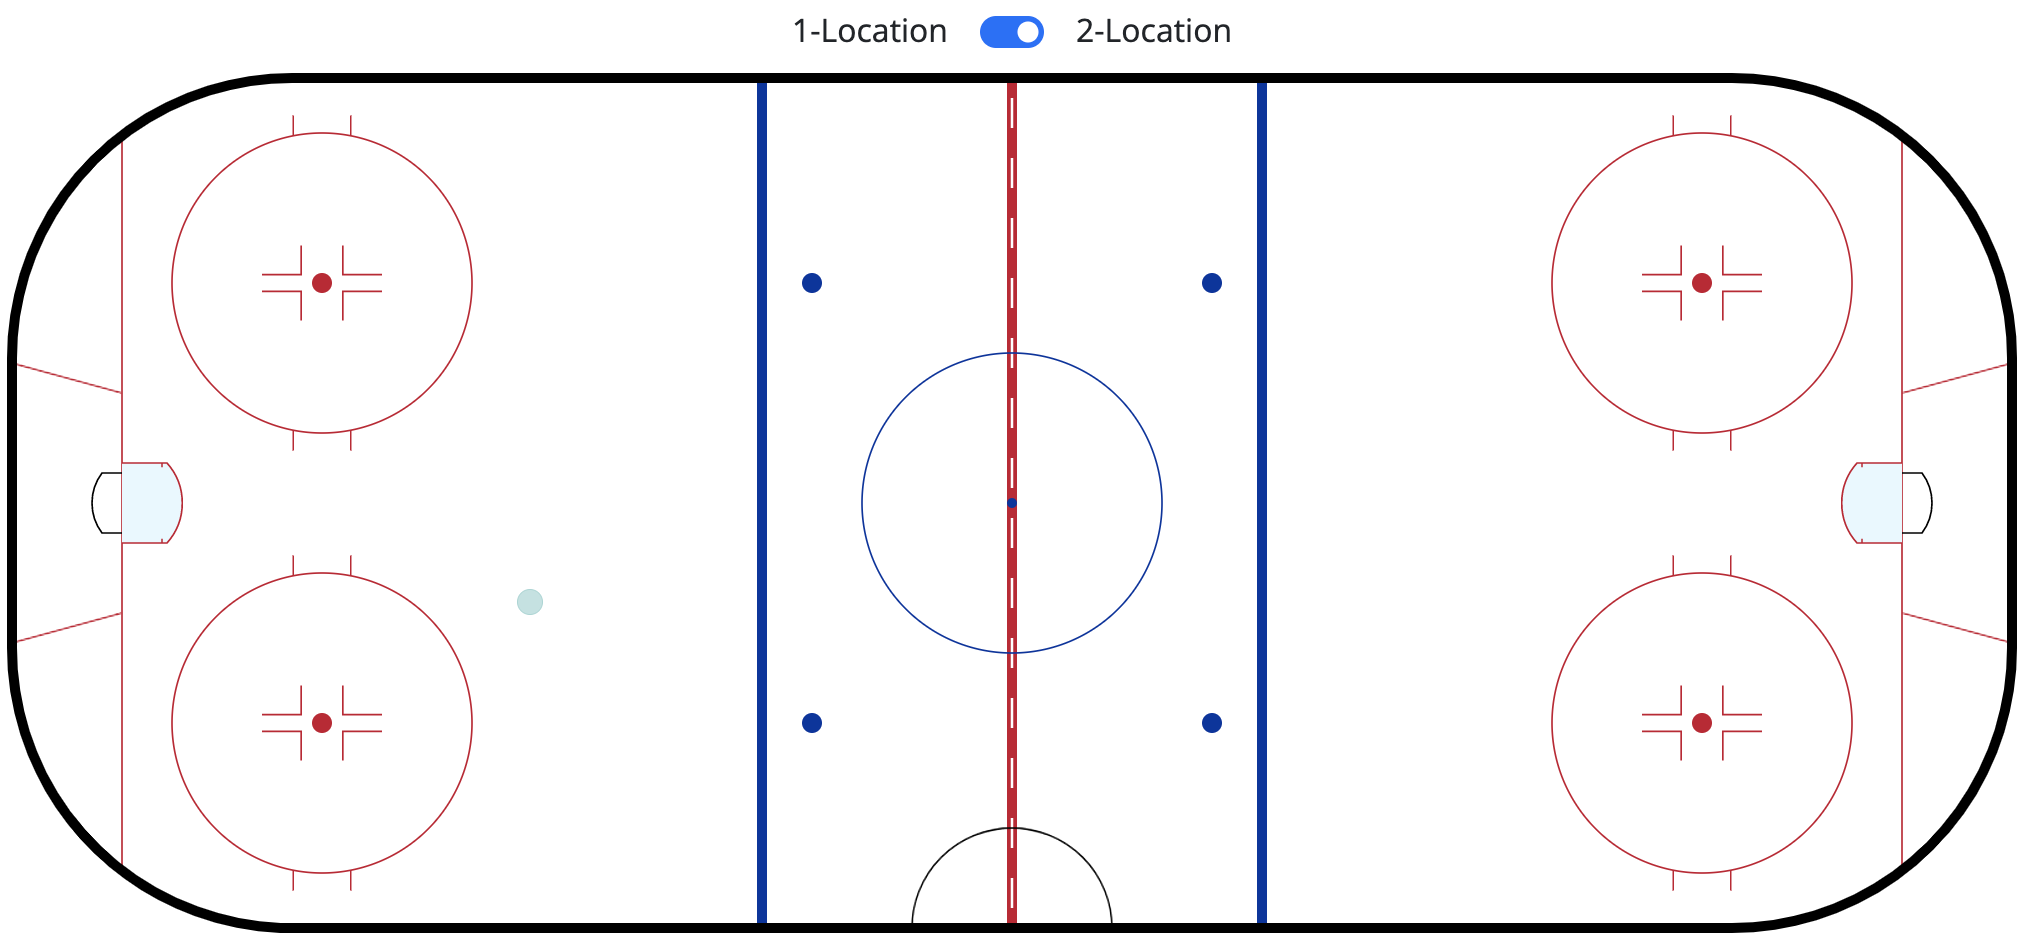
\includegraphics[width=1\linewidth]{images/ghost-dot}
	\caption{A rink with a single location for a 2-location event marked.}
	\end{subfigure}
		\begin{subfigure}{.5\textwidth}
	\centering
	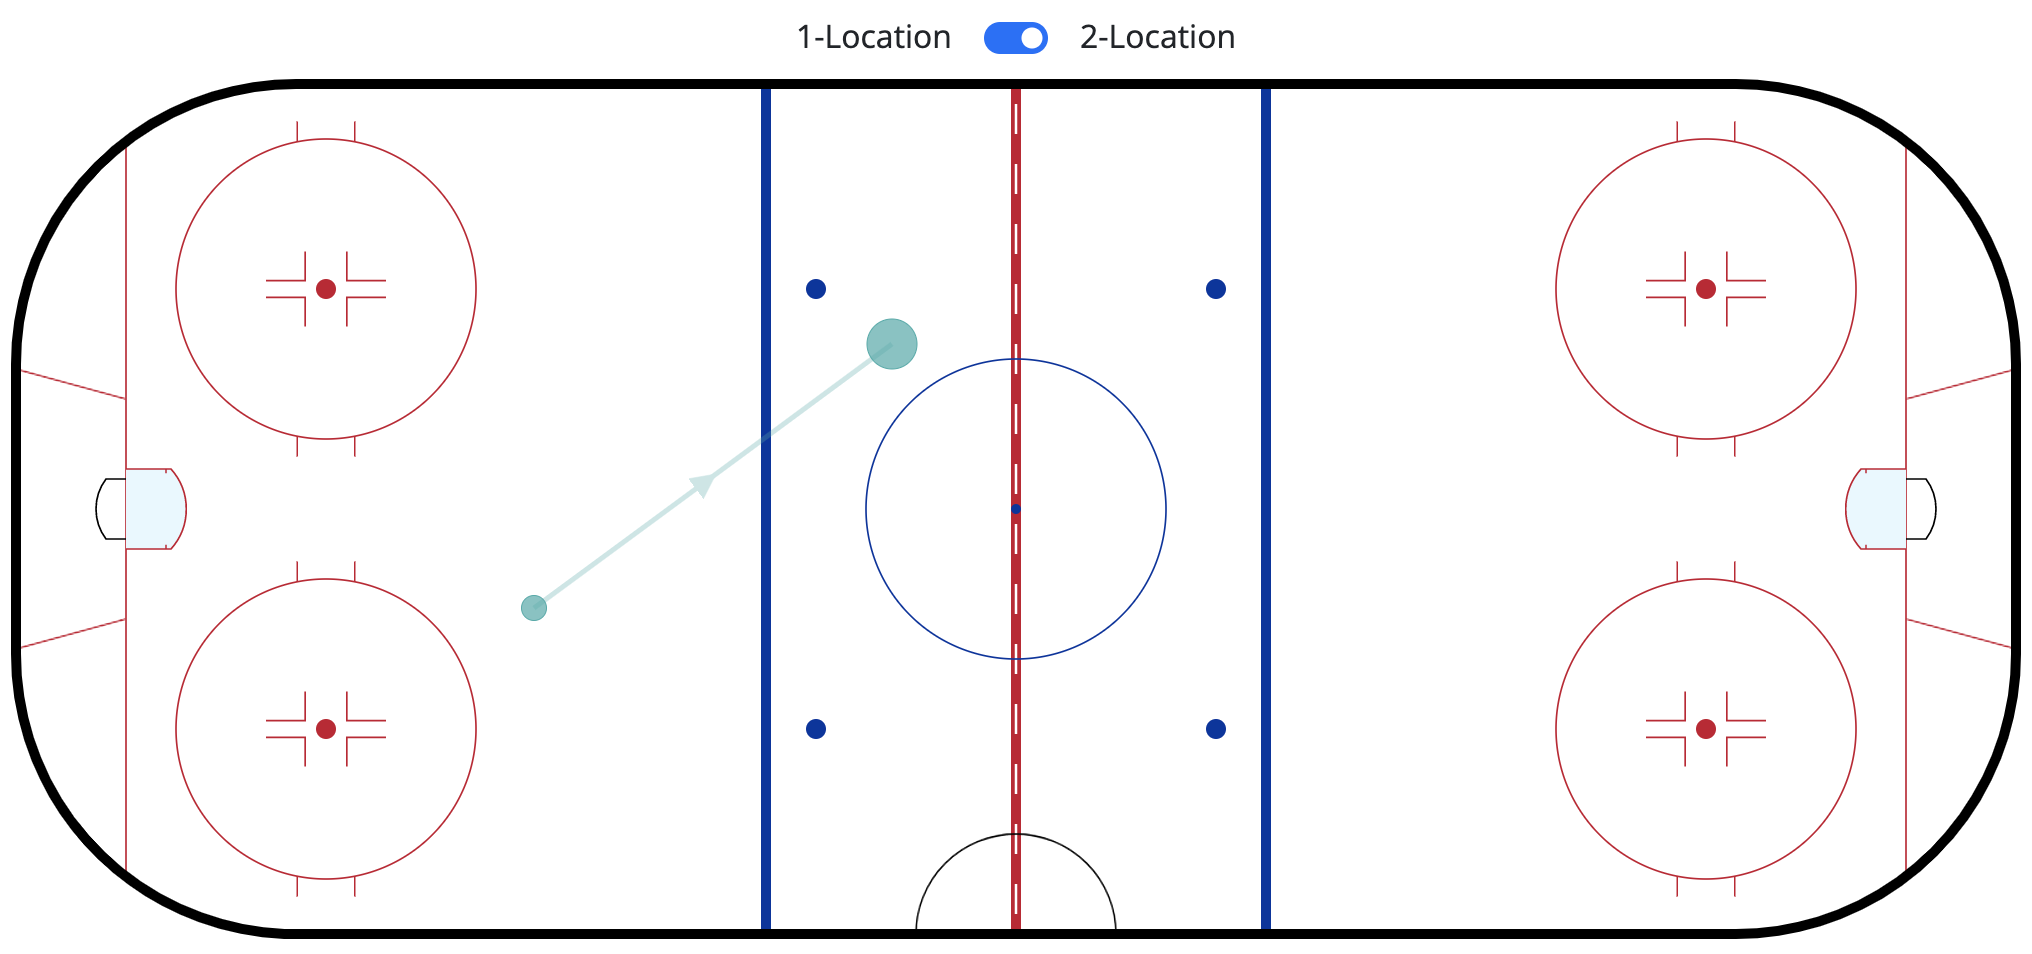
\includegraphics[width=1\linewidth]{images/two-location}
	\caption{A rink with a complete 2-location event logged.}
\end{subfigure}
\caption{The stages of logging a two-location event on the rink. The toggle between "1-location" and "2-location" mode above the rink is visible.}
\label{fig:two-location}
\end{figure}

Say we want to record an event best described using two locations: for example, passes with a start and endpoint. By enabling 2-location events, we can have two sets of coordinates for a single event

Enabling the "Enable 2-Location Events" option adds two details representing the coordinates for the new location: \textbf{X2} and \textbf{Y2}. As coordinate details, they cannot be hidden or deleted.

When we return to the main web application, besides the new \textbf{X2} and \textbf{Y2} columns in the table, above the rink there will be a similar toggle with values "1-location" and "2-location" (Figure \ref{fig:two-location}). This toggle indicates what type of event will be created. There are two ways to switch between the modes: the \textsc{shift} button on the keyboard and the toggle above the rink. "2-location" mode is active as long as the \textsc{shift} button is held down; this simplifies actively switching between the two modes. Alternately, clicking the toggle above the rink switches between the two modes. The toggle is useful for being in "2-location" mode for long periods without needing to hold down \textsc{shift} the entire time, and for mobile devices when the \textsc{shift} button is not present or not easily accessible.

In "1-location" mode, the application works as default, and the \textbf{X2} and \textbf{Y2} will be empty for all events. In "2-location" mode, clicking on the rink will first create a miniature, less opaque version of the traditional dot at that location. Then, clicking on the rink again will create a dot at this second location, with a line and an arrow connecting the two dots and the normal opacity for both dots (Figure \ref{fig:two-location}). Events are not logged in the table until both locations are marked. The first location, indicated by the smaller dot, has its coordinates in the  \textbf{X} and \textbf{Y} columns, while the second location, indicated by the normal-sized dot, has its coordinates in the \textbf{X2} and \textbf{Y2} columns.
 
\subsection{Setup Download and Upload} \label{setup-download-upload}
By creating new details and deleting and hiding unnecessary ones, changing the application's appearance, and enabling 2-location events, we can completely customize our setup of the application. However, those changes do not last forever; the application completely resets to default once refreshed to help ensure data privacy. But recreating a custom setup by hand is tedious at best and requires photographic memory at worst. 

Instead, next to the "Save Changes" button in the customization pop-up window, we can download a \texttt{.json} file. This file preserves the following information about the application's current setup: the current values of all widgets in the details panel, appearance preferences, whether 2-location events are enabled, and the order and visibility status of all details, including created details. Then, by uploading that same file at a later point in the upload section, that setup is completely restored. We can rename the file, by default named \texttt{custom-setup.json}, by clicking on the text box next to the download button.

For example, say we wanted to track passes during a series of games involving Finland. Before the series starts, we could make our custom setup. We could enable 2-location events, create any new details like perhaps a \textbf{Period Time} detail with a time widget, and hide and rearrange the columns. We could then hit "Save Changes" and modify the default values in the details panel, like by making Finland one of the \textbf{Team} options and adding any values to \textbf{Shot} we want, like whether an event went through "Traffic." Then, we can reopen the customization pop-up window since we haven't logged any events, and we can download our new custom setup file. Then, when we are about to track a game, we can open \textit{Shot-Plotter}, open the customization pop-up window, upload that file, and our changes will be restored. This custom setup \texttt{.json} file can also be shared with others to maintain a consistent data format for a larger-scale manual tracking project.

\section{Conclusion}
This application provides a user-friendly way to track events in ice hockey. The user interface guides input through form elements and icons, and makes logging events require as few clicks as possible with instant feedback about what was recorded. The application is currently known as \textit{Shot-Plotter} due to its default setup aimed at tracking shots, but its customizability allows almost any event imaginable to be easily tracked through the creation of custom details and 2-location events. The application benefits from active development: none of the customization features were available at the initial release in early April 2021 and have instead been added over time. There are many more planned features as well, like the ability to filter displayed events for using the rink as a live visualization tool. The application can aid the manual tracking of data in all levels of ice hockey, whether by independent fans and analysts or by ice hockey teams. In addition, the modular nature of the source code (available on \href{https://github.com/nguyenank/shot-plotter}{GitHub}) means the application could be adapted for other sports with relative ease. By swapping out the rink for an appropriately scaled \texttt{.svg} of another playing area and changing the default details, stored as a \texttt{.json}, the application could be used in other sports without touching the bulk of the code logic. 

By providing an easier way to track locational events, this application hopes to encourage manual tracking of data across leagues and levels, to increase the depth and breadth of high-quality and accessible data in ice hockey and, perhaps in the future, across the sports world in general.


\printbibliography
\end{document}
